\chapter{研究现状} \label{chap:related}
%本文根据在视频目标跟踪中使用方法的不同,将视频目标跟踪方法分为传统的基于相关滤波的视频目标跟踪方法和基于深度学习的视频目标跟踪方法。
%其中,基于相关滤波的视频目标跟踪方法本质上采用岭回归学习,由于其使用循环移位的特殊采样方式,可以通过快速离散傅里叶变换在频域中高效求解,具有较快的运行速度,成为了深度学习时代之前最具代表性的视频目标跟踪算法。
近年来,深度学习方法在视频目标跟踪任务中的应用越来越广泛。基于深度学习的视频目标跟踪方法,尤其是基于卷积神经网络的视频目标跟踪方法,受到学术和工业界的广泛关注。
%接下来,本章将分别对传统的基于相关滤波的视频目标跟踪方法和基于深度学习的视频目标跟踪方法进行系统的介绍。
本章主要介绍基于深度学习的目标跟踪的研究现状,将基于深度学习的跟踪器划分为以下几种类别:基于深度特征的相关滤波跟踪器、基于生成对抗网络的跟踪器、基于图卷积网络的跟踪器、基于循环神经网络的跟踪器、基于脉冲神经网络的跟踪器、基于孪生网络的跟踪器、基于强化学习的跟踪器、基于元学习的跟踪器、基于无监督学习的跟踪器、基于注意力机制的跟踪器和基于串并联或级联结构的跟踪器。

\section{基于深度特征的相关滤波跟踪器}
相关滤波跟踪器是传统跟踪器中的代表之一。基于相关滤波的视频目标跟踪方法本质上采用岭回归学习,由于其使用循环移位的特殊采样方式,可以通过快速离散傅里叶变换在频域中高效求解,具有较快的运行速度,成为了深度学习时代之前最具代表性的视频目标跟踪算法。
%相关滤波跟踪的基本思想是,设计一个滤波模板,利用该模板与目标候选区域做相关运算,最大输出响应的位置即为当前帧的目标位置。该跟踪器通过利用离散傅立叶变换以有效的方式利用了跟踪样本的所有空间偏移。
%基于相关滤波的视频目标跟踪算法将空域内的密集搜索通过相关滤波的方式转化为频域内的点积运算,得益于快速傅里叶变换,在频域内高效进行表观建模,跟踪实时性好,能够达到很高的帧率。
Bolme 等 \cite{MOSSE} 首次将相关滤波于自适应目标跟踪相结合,提出 MOSSE 跟踪算法,该跟踪器以每秒 669 帧的速度运行,可以抵抗光照,比例,姿势和非刚性变形的变化。
CSK 跟踪器 \cite{Henriques2012ExploitingTC} 通过采用图像子窗口的循环结构并使用快速傅里叶变换(FFT)快速合并来自所有子窗口的信息,对 MOSSE 跟踪器进行了改进。此外, \cite{Henriques2012ExploitingTC} 表明,使用核技巧可以像在原始图像空间中一样高效地完成非线性空间中的分类。
\cite{Danelljan2014AdaptiveCA} 通过学习有关多维颜色属性的多通道滤镜来改进 CSK 跟踪器。为了避免由于颜色属性的高维而导致的计算开销,\cite{Danelljan2014AdaptiveCA} 提出了一种自适应维降技术,可以将原始的 11 维减少到只有 2 维。
后来,\cite{henriques2014high-speed} 为成千上万个已翻译补丁的数据集提出了一种分析模型。使用离散傅立叶变换将模型对角线化。此操作可以将存储和计算量减少几个数量级。

传统的相关滤波跟踪器通常采用手工设计的特征或底层特征,这限制了相关滤波器的潜力。随着深度学习时代的到来,有很多相关滤波跟踪器尝试使用深度特征代替底层特征,并取得了性能的提升。\cite{CF2} 利用从深度卷积神经网络中提取的特征进行相关滤波的学习,来提高跟踪精度和鲁棒性。作者利用最后一个卷积层的输出对目标的语义信息进行编码,使得跟踪器对于目标的表观变化具有鲁棒性。但是,由于空间分辨率太粗糙,无法精确定位目标。相反,较浅的卷积层提供了更精确的定位。因此作者在每个卷积层上自适应学习相关滤波器,以对目标表观进行编码。在 \cite{danelljan2016beyond} 中,作者在常规相关滤波跟踪器框架的基础上,提出了一种用于训练连续卷积滤波器的算法。作者采用隐式插值模型来解决连续空间域中的学习问题。该模型可实现对于多种分辨率的特征图的有效集成。此外,该方法能够进行亚像素定位,有利于提高跟踪的精确性。
\section{基于生成对抗网络的跟踪器}
生成对抗网络(GAN)可以通过 CNN 从随机噪声生成逼真的图像。 生成对抗网络包含两个子网,一个充当生成器,另一个充当判别器。 生成器旨在合成图像以欺骗判别器,而判别器则试图正确区分真实图像和生成器合成的图像。通过相互竞争来同时训练生成器和鉴别器。对抗学习的优势在于,所训练的生成器可以生成与训练样本相似的图像统计信息,从而使判别器无法区分。生成对抗网络的进步吸引了包括目标跟踪在内的各种计算机视觉应用的关注。在 \cite{VITAL} 中,作者利用生成对抗网络产生的样本辅助跟踪器的学习。文章指出,由于以下问题,现有视觉跟踪器的性能可能会受到限制:i)采用密集采样策略生成的正样本会降低样本的多样性;ii)即使收集到大规模的训练数据集,具有挑战性的训练数据也是有限的。作者提出了 VITAL 算法来通过对抗学习解决这两个问题。为了增加正样本,作者使用一个生成网络随机生成模板,这些模板用于自适应过滤输入特征以捕获各种表观变化。通过对抗学习获得的模板,可以提供最鲁棒的目标特征。此外,为了解决类别不平衡的问题,作者提出了一个高阶成本敏感损失,从而有助于训练分类网络。在 \cite{SINT++} 中,作者通过对抗生成学习产生难例正样本进行跟踪。具体来说,作者假设目标都位于流形上,因此,引入正样本生成网络(PSGN),通过遍历已构建的目标流形来采样大量训练数据。生成的各种目标图像可以丰富训练数据集并增强目标跟踪器的鲁棒性。为了使跟踪器对遮挡更加鲁棒,作者提出了一个变换网络,该网络可以生成用于跟踪算法的难例样本。%SINT++: robust visual tracking via adversarial positive instance generation
受生成对抗网络(GAN)\cite{GAN} 和条件 GAN(cGAN)\cite{cGAN} 启发, \cite{AdversarialDeep} 提出了一种跟踪器,其中通过对抗学习共同优化了回归 CNN(R-Net)和分类 CNN(C-Net)。在训练阶段,我们分别为 R-Net 和 C-Net 创建元组和三元组训练集。元组训练集包含目标补丁和搜索补丁。通过元组训练集,可以训练 R-Net 生成一个响应图,该图反映目标在搜索补丁中的位置和大小。三重训练集包含目标的模板补丁,搜索补丁和响应图。通过三重训练集,对 C-Net 进行了训练,以区分响应图是否可以反映搜索补丁中模板补丁中目标的位置和大小。在测试阶段,我们在当前帧周围的目标位置出现在最后一帧中提取了几个搜索补丁作为候选。元组集包含一个搜索补丁和一个目标补丁。 R-Net 基于这些元组集生成一组响应图。然后,C-Net 根据三元组来区分哪个响应图是最好的。最后,我们使用最佳响应图在当前帧中定位目标。  % Adversarial Deep Tracking

\section{基于图卷积网络的跟踪器}
图卷积神经网络(Graph Convolutional Network)是一种能对图数据进行深度学习的方法。在目标跟踪中,图卷积网络用于捕获目标样本的结构特征。在 \cite{gao2019graph} 中,作者指出时空信息可以用于增强目标表示,并且上下文信息对于目标的定位很重要。为了全面利用历史目标样本的时空结构并从上下文信息中受益,作者提出了一种用于高性能视觉跟踪的新型图卷积跟踪(GCT)方法。具体而言,GCT 将两种类型的图卷积网络(GCN)合并到用于目标表观建模的孪生框架中。作者采用时空GCN来建模历史目标样本的结构化表示。而上下文 GCN 被设计为利用当前帧的上下文来学习用于目标定位的自适应特征。在 \cite{tu2019visual} 中,作者同样使用GCN模块来学习目标跟踪的结构特征。首先,作者利用双路径网络提取异构特征。然后,作者采用GCN模块来构建具有结构化信息的要素。
\section{基于循环神经网络的跟踪器}
循环神经网络(Recurrent Neural Network, RNN)是一类以序列(sequence)数据为输入,在序列的演进方向进行递归(recursion)且所有节点(循环单元)按链式连接的神经网络。RNN 在建模序列数据方面引起了越来越多的关注。这些应用程序涵盖了多语言机器翻译,动作识别,场景标记,语音识别等。最近,传统的 RNN 被归纳为更复杂的结构模型,例如二维 RNN [17,18],多维 RNN [19,20,21],树 RNN [22,23]等。在目标跟踪中,可利用RNN建模目标的复杂远程依赖关系。
RTT[24]尝试识别并利用那些对整个跟踪过程有益的可靠部分。为了解决遮挡并发现可靠的组件,RTT中使用了多方向递归神经网络,通过从多个方向遍历候选空间区域来捕获远程上下文线索。从RNN生成的置信度图用于抑制背景噪声,同时充分利用来自可靠部分的信息,来自适应地区分判别相关滤波器的学习。%Recurrently target-attending tracking
在 \cite{SpatiallySupervised} 中,我们的循环卷积网络利用位置的历史以及由深度神经网络学到的独特视觉特征。受最近用于对象检测的边界框回归方法的启发,我们研究了时域中的长短期记忆(LSTM)的回归能力,并提出了将卷积网络产生的高级视觉特征与区域信息连接起来的方法。与将二进制分类用于区域候选的现有基于深度学习的跟踪器不同,我们使用回归来直接预测卷积层和循环单元处的跟踪位置。与仅基于位置历史的基于卡尔曼滤波器或相关时间预测方法的现有跟踪方法相比,我们的循环卷积模型具有“双重深度”,因为它可以检查位置的历史以及过去帧的鲁棒视觉特征。% spatially supervised recurrent convolutional neural networks for visual object tracking
在[25]中,作者提出了一种能够将时间信息整合到模型中的实时目标跟踪器。该跟踪器不是专注于有限的一组目标或在测试时训练一个模型来跟踪特定的实例,而是在大量不同的目标上预先训练一个通用跟踪器,并进行实时的在线更新。%Re al-Time Recurrent Regression Networks for Visual Tracking of Generic Objects
\cite{RecurrentFilter} 通过保持目标外观并通过长期短期记忆(LSTM)网络跟踪过滤器,提出了循环过滤器学习(RFL)算法。 全卷积神经网络用于编码目标外观信息,同时保留目标的空间结构。 天真地将CNN特征图展平为向量,以便将其传递给LSTM,这会使目标的结构变得模糊。 相反,受[37]的启发,我们将LSTM的输入,输出,单元和隐藏状态更改为特征图,并使用卷积层而不是完全连接的层。 卷积LSTM的输出本身就是一个滤波器,然后将其与下一帧的特征图进行卷积以生成目标响应图。%Recurrent Filter Learning for Visual Tracking
\cite{PRNet} 整个图像中不同比例的上下文提供了不同的空间关系线索,应该以适当的方式充分利用它进行视觉跟踪。为了纳入全面的上下文线索,我们提出了金字塔递归网络(PRNet)。在每种上下文比例中,建议使用多达8个方向的RNN来收集目标的上下文信息。每个定向RNN都可以提取目标各部分之间的上下文相关性,这使其不仅对背景对象而且对相似的干扰项也更具区分性。 % Multi-Scale Recurrent Tracking via Pyramid Recurrent Network and Optical Flow
\section{基于脉冲神经网络的跟踪器}% SiamSNN: Spike-based Siamese Network for Energy-Efficient and Real-time Object Tracking
脉冲神经网络(spiking neural network,SNN)深层神经网络(DNN)在各种情况下均表现出卓越的性能[1],[2],[3]。然而,由于高计算成本和高能耗,难以在诸如移动设备之类的嵌入式系统上使用DNN。为此,提出了许多微小但有效的网络[4],[5],并实现了有希望的性能。但是,资源有限的系统中仍然存在计算能力不足的问题。作为替代方案,尖峰神经网络(SNN)通过以事件驱动的二进制峰值序列而不是连续的形式传输信息来实现神经形态硬件(例如TrueNorth [6]和Loihi [7])上的超低功耗。值,例如DNN [8]。此外,SNN中的尖峰神经元仅在其膜电位超过特定阈值时才触发输出尖峰[9],这会稀疏地激活网络中的神经元以节省能量。 SNN被视为第三代人工神经网络。
最新的跟踪模型[26],[27]需要高性能的GPU,这会导致计算和功耗需求的急剧增加,而这对于嵌入式平台来说是很难解决的[28]。借助SNN中的节能计算,实现基于尖峰的跟踪器对于在嵌入式系统上实现节能跟踪算法具有重要意义。\cite{SiamSNN} 我们设计了SiamSNN用于深度SNN中的对象跟踪,且延迟短且精度损失低。这是将深度SNN应用于具有复杂场景的数据集上的对象跟踪的首次成功尝试。 •我们利用尖峰序列的时间信息,并提出了一种优化的混合相似度估计方法来构建基于尖峰的相关层,该层可以以尖峰方式有效地评估两个特征图之间的相似度。 •我们提出了一种新颖的编码方案来优化输出尖峰序列的时间分布,从而改善性能并缩短等待时间。
\cite{DashNet} 用于SNN跟踪的直接培训方法。我们为基于事件驱动的数据集开发了SNN模型,并为跟踪提供了准确的信息表示。据我们所知,这是探索针对跟踪和检测任务的SNN直接培训的第一项工作。 •用于高速跟踪的混合人工和峰值模型。我们提出一种混合模式,通过TCF和注意力机制共同处理来自ANN的同步信号和来自SNN的事件驱动信号。随后,它在神经形态芯片上获得了最佳性能和创纪录的2083 FPS跟踪速度。%https://arxiv.org/pdf/1909.12942.pdf
\section{基于孪生网络的跟踪器}
孪生网络是一种用于度量学习的有监督模型。孪生网络具有两个参数共享的子网络,可以学习两幅输入图像之间的特征相似性。由于优越的性能,基于孪生网络的跟踪器已经成为当前目标跟踪领域的主流。在SiamFC[26]中证明了使用孪生网络解决跟踪问题的有效性。具体来说,作者训练了一个孪生网络以在较大的搜索图像中定位模板图像。利用互相关操作以滑动窗口的方式获得目标位置的响应图,从而对目标进行实时定位。在SiamRPN[27]中,跟踪器由用于特征提取的孪生网络和包括分类分支和回归分支的region proposal子网络组成。受益于跟踪器的改进,传统的多尺度测试和在线微调可以被丢弃。SiamRPN++ \cite{SiamRPN++} 基于其在分类和状态估计分解中的成功经验,通过一种简单而有效的空间感知采样策略进一步突破了严格的翻译不变性的限制,并成功地训练了 ResNet 驱动的孪生跟踪器,从而显着提高了性能。除了这些基于锚的方法以外,还通过考虑无歧义评分,无目标目标规模/比率分布和估计质量评估准则,进一步设计了无锚跟踪器 SiamFC++ \cite{SiamFC++}。
\subsection{针对孪生网络跟踪器的对抗攻击}
广泛的研究表明,卷积神经网络容易受到对抗攻击 \cite{Deepsec}。\cite{intriguing} 最初显示了对抗性攻击的存在,\cite{FGSM} 提出了一种有效的单步方法FGSM,后来通过迭代方法 \cite{kurakin2017adversarial} 和动量项 \cite{dong2018boosting} 进行了改进。同样,\cite{papernot2016limitations} 提出了基于雅可比的显着性图攻击,成功率很高,而 \cite{carlini2017towards} 通过优化方法(C&W)在不同规范下实现了有效攻击。 进一步的对抗攻击扩展到诸如自然语言处理 \cite{generating} 和图像目标检测 \cite{wei2019transferable}之类的任务。
最近有研究表明,基于卷积神经网络的孪生跟踪器同样容易受到对抗攻击。\cite{SPARK} 正式确定了视频目标跟踪的对抗性攻击问题,即,在线生成无法察觉的扰动,以误导跟踪对象的视觉跟踪器,使其成为不正确的(非目标攻击,UA)或指定的(目标攻击) ,TA)轨迹。提出了一种空间感知的在线增量攻击(SPARK)方法,该方法可以在有效性和效率上在线产生更多难以察觉的扰动。SPARK \cite{SPARK} 通过使用过去帧中的信息对孪生跟踪器进行有针对性的攻击来计算增量扰动。但是,SPARK 需要通过繁琐的迭代方案为每个搜索图像生成独特的对抗示例,这对于实时攻击在线跟踪非常耗时。\cite{chen2020one} 探索了一种具有双重损失和双重关注机制的新颖攻击方法,以在初始帧处对目标补丁产生对抗性干扰。我们提出的攻击方法的优化目标包括两个部分,每个损失都与相应的精心设计的关注权重相结合,以进一步提高攻击能力。
例如,PAT \cite{PAT} 通过白盒攻击生成物理对抗纹理,以引导跟踪器在被跟踪对象移到其前面时锁定该纹理。但是,PAT 通过攻击轻型深度回归跟踪器 GOTURN \cite{GOTURN} 来验证其方法,该跟踪器在现代基准上的跟踪精度较低。在本文中,我们旨在攻击最先进的孪生跟踪器。
在估计的跟踪结果中逐帧生成轻量级扰动时,RTAA \cite{RTAA} 考虑到了时间运动。但是,RTAA 仅对跟踪器执行无目标攻击,这比本文中的有针对性的攻击更具挑战性,因为我们的目标是在测试时创建任意的复杂轨迹。

遵循看起来真实的错误路径进行有针对性的攻击对于欺骗跟踪系统而不会引起现实应用程序的怀疑至关重要。
\cite{TTP} 中最近的实时攻击者仅使用模板图像以一次生成的方式生成时间可传递的扰动,然后将其添加到每个搜索图像中。但是,该方法仍然需要为每个视频生成扰动,并且其有针对性的攻击设置需要从网络推理的多次运行中获得不同的扰动。当我们无法访问有限的计算资源时,就不适合攻击现实世界的在线跟踪系统。
\section{基于强化学习的跟踪器}
强化学习(RL)的目标是学习一种通过最大化未来累积奖励来决定动作序列的策略。
在[28]中,作者提出了一种新颖的跟踪器,该跟踪器顺序执行通过深度强化学习而学到的动作来进行控制。与使用深层网络的现有跟踪器相比,所提出的跟踪器旨在实现轻量级计算以及令人满意的跟踪精度。控制动作的深层网络使用各种训练序列进行了预训练,并在跟踪过程中进行了微调,以在线适应目标和背景变化。 %  Action-decision networks for visual tracking with deep reinforcement learning
在[29]中,作者将跟踪形式化为部分可观察的决策过程(POMDP)来学习最佳决策策略。作者使用深度强化学习算法学习策略,这些算法仅在运动轨迹出现问题时才需要监督(奖励信号)。作者证明稀疏的奖励有利于快速地对海量数据集进行训练。 %  Tracking as online decision-making: Learning a policy from streaming videos with reinforcement learning
在 \cite{DeepReinforcement} 中,跟踪问题可以看作是一个顺序决策过程,而历史语义编码了与将来决策密切相关的信息。基于这种直觉,我们将模型表示为与视频超时互动的循环卷积神经网络代理,并且可以使用强化学习(RL)算法对模型进行训练,以学习关注连续,跨帧的良好跟踪策略相关性并从长远来看最大化跟踪性能。我们的跟踪器是首个将卷积和递归网络与RL算法结合在一起的神经网络跟踪器。% Deep Reinforcement Learning for Visual Object Tracking in Videos
在 \cite{RealTimeVisual} 中,介绍了一种基于深度强化学习方法构造的模板选择策略的新型实时视觉跟踪算法。跟踪算法利用此策略来选择适当的模板以跟踪给定的帧。模板选择策略是通过对跟踪基准数据集中随机生成的大量训练情节使用简单的策略梯度方法来自学习的。% Real-time visual tracking by deep reinforced decision making
在 \cite{HierarchicalTracking} 中,从深度递归强化学习中学到的数据驱动运动模型为跟踪器提供了对象的粗略定位。通过将运动搜索表述为强化学习中的动作决定问题,我们的跟踪器利用基于循环卷积神经网络的深度Q网络来有效地学习数据驱动的搜索策略。在每一帧中,我们的运动模型将以先前估计位置为中心的候选图像块迭代地作为输入,并生成每个动作的概率作为输出。在每次迭代中,选择一个最佳动作来移动目标边界框。减少搜索步骤。学习的运动模型不仅可以大大减少搜索空间,而且可以提供更可靠的感兴趣区域以进行进一步验证。% Hierarchical Tracking by Reinforcement Learning-Based Searching and Coarse-to-Fine Verifying
在 \cite{LearningPolicies} 中,我们将自适应跟踪问题公式化为决策过程,并学习一个代理来决定是否以较高的置信度在早期层上定位对象,或者继续处理网络的后续层。对于具有不同物体或移动缓慢的物体的简易镜架,这大大降低了前馈成本。具体来说,该代理学习在每一层上找到目标,并确定是否有足够的信心在此处输出和停止。如果没有,它将前进到下一层继续。这等效于学习“及时的”决策策略以选择最佳层进行跟踪。我们将显示,这种策略学习比启发式阈值当前活动层的响应图要强大得多。我们以强化学习的方式对代理进行离线培训,并进一步证明学习所有深层(以便为自适应跟踪提供良好的功能)可以在达到状态的同时在单个CPU上实现接近23 fps的实时平均跟踪速度最先进的性能。% Learning Policies for Adaptive Tracking with Deep Feature Cascades
\section{基于元学习的跟踪器} %https://openaccess.thecvf.com/content_CVPR_2020/papers/Wang_Tracking_by_Instance_Detection_A_Meta-Learning_Approach_CVPR_2020_paper.pdf
元学习的目标是针对各种学习任务训练模型,以便仅使用少量训练样本即可解决新的学习任务[10]。当我们将对象跟踪视为实例检测任务时,跟踪器将接受各种实例检测任务的培训,以便它可以仅使用来自初始或先前帧的一个或几个训练样本就可以快速学习如何检测新实例。我们发现跟踪任务是应用元学习的完美示例。与模型无关的元学习(MAML)[10]是元学习的重要算法。它有助于网络学习一组适用于微调的良好初始化参数。在训练期间,显式训练模型的参数,以使少量梯度步骤和来自新任务的少量训练数据将对该任务产生良好的泛化性能。 MAML最引人注目的优点是,它与通过梯度下降训练的任何模型兼容,并且适用于各种不同的学习问题。因此,MML是实现我们的想法的理想人选,该想法是将任何高级对象检测器(经过梯度下降训练)转换为跟踪器。后来,MAML ++ [1]引入了一些技巧来稳定MAML的训练。 MetaSGD [23]建议针对每个参数训练可学习的学习率。在对象跟踪领域,Meta-Tracker [29]率先将MAML用于MDNet的域自适应步骤。建议使用未来帧中的错误信号。在元训练阶段,我们旨在找到通用的初始表示形式和渐变方向,以使目标模型能够专注于对未来框架有用的特征。同样,此元训练阶段有助于避免在当前帧中过度适应干扰项。此外,通过在元训练期间强制执行更新迭代次数,可以在初始化期间显着加快训练结果网络的速度。我们提出的方法可以稍加修改即可应用于任何基于学习的跟踪器。我们从基于分类器的跟踪器(按检测跟踪)类别中选择两个最新的跟踪器MDNet [1],以及基于相关性的跟踪器CREST [2]。实验结果表明,这些跟踪器的元学习版本可以非常快速地(仅一次迭代)适应第一帧,同时提高了准确性和鲁棒性。请注意,即使没有采用某些手工设计的训练技术,复杂的建筑设计以及原始跟踪器的超参数选择,也可以完成此操作。简而言之,我们提供了一种简单的方法,无需过多的努力就可以使出色的跟踪器变得更好,并在两种不同的跟踪体系结构上展示其成功,表明其潜在的普遍适用性。 MetaRTT [16]进一步将MAML应用于在线更新步骤。基本上,它们的主要目的是加速现有跟踪器的在线培训,包括MDNet [28],CREST [31]和RTMDNet [15]。我们认为,由于元学习提供了一种快速适应深度网络以对特定对象建模并避免过度拟合的机制,为什么不直接将现代对象检测器转换为跟踪器,而不是使慢速跟踪器更快?[13]有相同的想法。他们建议将跟踪作为单发对象检测和少发实例分类的联合任务,并且我们提出了一个高效的目标指导模块和一个元学习器来处理各个子任务。通过MAML学习检测头中的元层。但是,他们仍在跟踪器的第一部分中引入了一个称为类级对象检测的模板。复杂的设计导致速度慢。在 \cite{TrackingBy} 中,提出了一种原则性的三步方法来构建高性能跟踪器。首先,选择任何经过梯度下降训练的现代物体探测器。其次,使用MAML进行离线培训(或初始化)。第三,使用初始帧执行域自适应。我们遵循此过程,基于两个现代检测器RetinaNet和FCOS构建两个名为RetinaMAML和FCOS-MAML的跟踪器。
\section{基于无监督学习的跟踪器}
无监督学习(unsupervised learning)是机器学习的一种方法,没有给定事先标记过的训练样本,自动对输入的数据进行分类或聚类。常见的目标跟踪方法往往需要以监督方式进行训练,需要大量带注释的真实标签。手动注释往往是昂贵且费时的,而大量的未标记视频可在Internet上轻松获得。通过无监督学习,可以利用未标记的视频序列进行视觉跟踪。在[30]中,作者通过使用辅助自然图像,离线训练堆叠式去噪自动编码器,以学习对变化更鲁棒的通用图像特征。然后,将知识从离线培训转移到在线跟踪过程。在线跟踪网络由训练过的自动编码器(作为特征提取器)和一个附加的分类层构成。特征提取器和分类器都可以进行在线更新以适应运动目标的表观变化。在[31]中,作者提出了一种无监督的视觉跟踪方法。与使用大量有标签数据进行监督学习的现有方法不同,作者提出的CNN模型是在无监督的大规模无标签视频上进行训练的。作者的动机是,强大的跟踪器在前向和后向预测中均应有效(即,跟踪器可以在连续帧中向前定位目标并回溯到其在第一帧中的初始位置)。作者在一个孪生相关滤波网络上构建跟踪框架,该网络使用未标记的原始视频进行训练。同时,文中提出了一种多帧验证方法和一种成本敏感的损失函数,以促进无监督学习。
\section{基于注意力机制的跟踪器}
注意力机制首先用于神经科学领域[32]。它们已经扩展到其他领域,例如图像分类[33,34,35],姿态估计[36]等。在目标跟踪领域中,注意力机制有利于使网络的学习关注更有效的信息。
在 \cite{RATM} 中,我们提出了一种基于注意力的用于计算机视觉的模块化神经框架。该框架使用一种软注意力机制,允许使用梯度下降来训练模型。它由三个模块组成:一个循环注意力模块,用于控制在图像或视频帧中的显示位置;一个特征提取模块,用于提供所见内容的表示形式;以及一个客观模块,用于规范该模型学习其注意行为的原因。注意模块允许模型将计算的重点放在输入中与任务相关的信息上。% RATM: Recurrent Attentive Tracking Model
RASNet模型[37]在孪生跟踪框架内重新构造了相关过滤器,并引入了各种注意机制来适应模型而无需在线更新模型。通过利用离线训练的通用注意力,目标自适应的残差注意力以及通道特征注意力,RASNet不仅减轻了深度网络训练中的过拟合问题,而且具有更强的判别能力和适应性,从而提高了跟踪的性能。文中提出的深度架构是端到端训练的,充分利用了丰富的时空信息来实现强大的视觉跟踪。在[38]中,作者提出了一种具有注意力机制的新型跟踪框架,该机制通过选择相关过滤器的子集以提高鲁棒性和计算效率。滤波器的子集由深度注意力网络根据目标的动态属性进行自适应选择。该算法的贡献主要有:(1)引入注意力相关过滤器网络,该网络可以自适应跟踪动态目标。(2)利用注意力网络将注意力转移到最佳候选模块,并预测当前非活动模块的估计准确性。(3)扩大了相关滤波器的种类,涵盖目标漂移,模糊,遮挡,缩放变化和灵活的宽高比。(4)通过大量实验验证了视觉跟踪注意机制的鲁棒性和效率。
\section{基于串并联或级联结构的跟踪器}
SPM-Tracker[39]的基本思想是在两个单独的匹配阶段解决两个需求。在粗匹配(CM)阶段,通过通用训练增强了鲁棒性,而在精细匹配(FM)阶段,通过在线学习,增强了网络辨别力。 FM阶段的输入区域由CM阶段生成,因此这两个阶段串联连接。同时,这两个阶段也被并行连接,因为匹配分数信息和目标边框位置信息被融合以生成最终结果。这种创新的串并联结构充分利用了两个阶段的优势,并具有出色的性能。在[40]中,作者指出,最近流行的SiamRPN目标跟踪器在存在表观近似的干扰目标和目标剧烈变化的情况下会退化。为了解决这些问题,作者提出了一个多阶段跟踪框架,即孪生级联RPN(C-RPN),该框架由一系列来自孪生网络中不同层次的RPN组合而成。与以前的解决方案相比,C-RPN具有几个优点:(1)每个RPN在上一阶段都使用RPN的输出进行训练。这样的过程会关注难分的负采样,从而使训练样本更加均衡。因此,RPN在区分困难的背景(即类似的干扰因素)时将更具区分性。(2)提出了特征转移块(FTB)以充分利用多级特征,从而进一步使用高级语义和低级空间信息来改善C-RPN的辨别能力。(3)通过多步回归,C-RPN在多个阶段逐步调整每个RPN中目标的位置和形状,从而使定位更加准确。
\begin{figure}
\centering
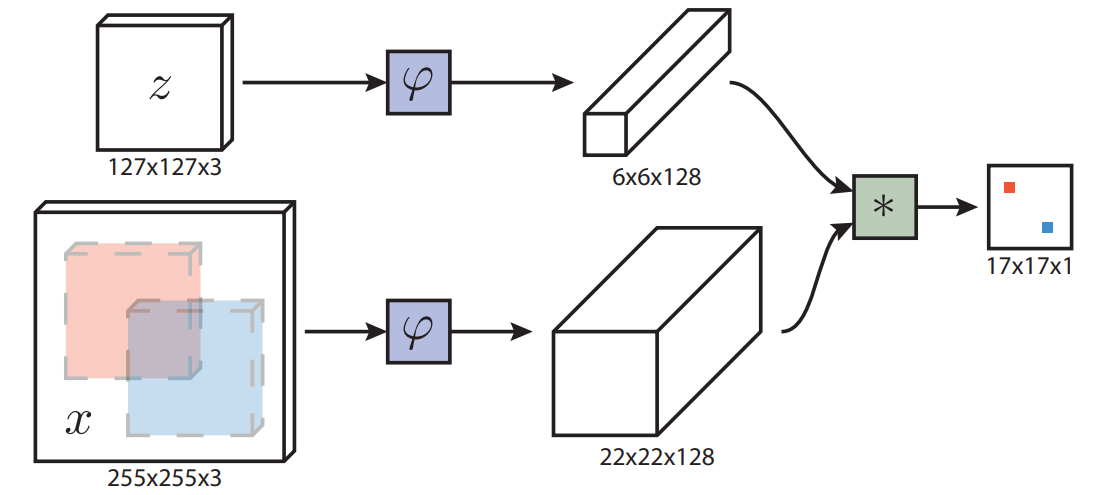
\includegraphics[width=0.75\textwidth]{Img/related/SiamFC.png}
\caption{SiamFC}
\end{figure}

\begin{figure}
\centering
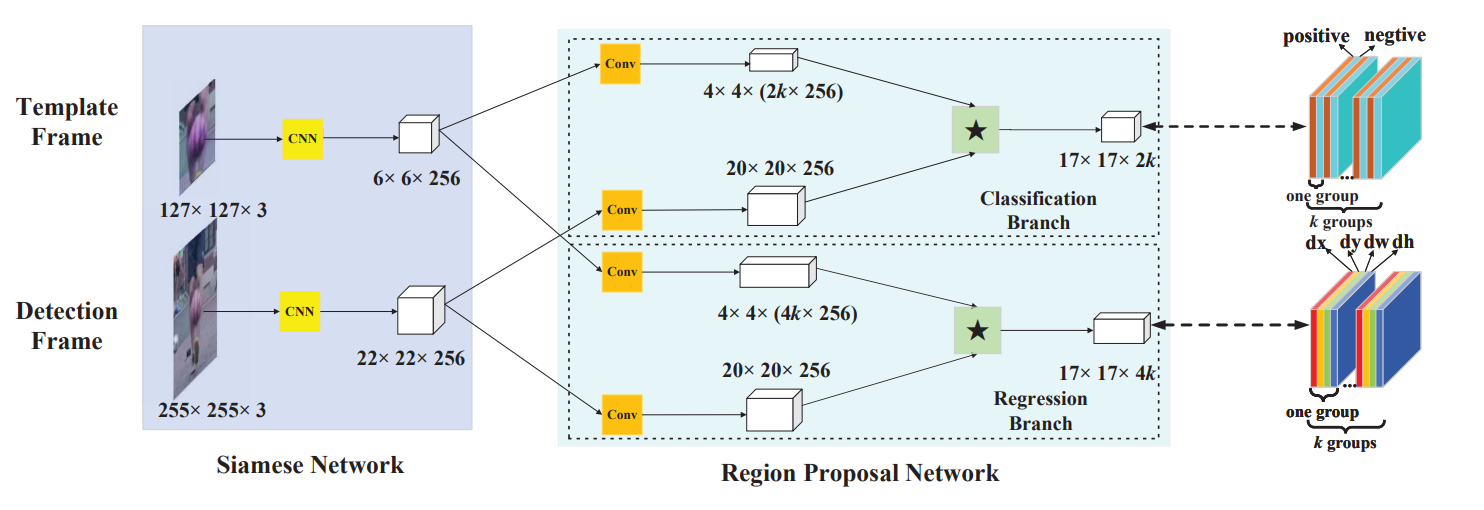
\includegraphics[width=0.75\textwidth]{Img/related/SiamRPN.png}
\caption{SiamRPN}
\end{figure}

\begin{figure}
\centering
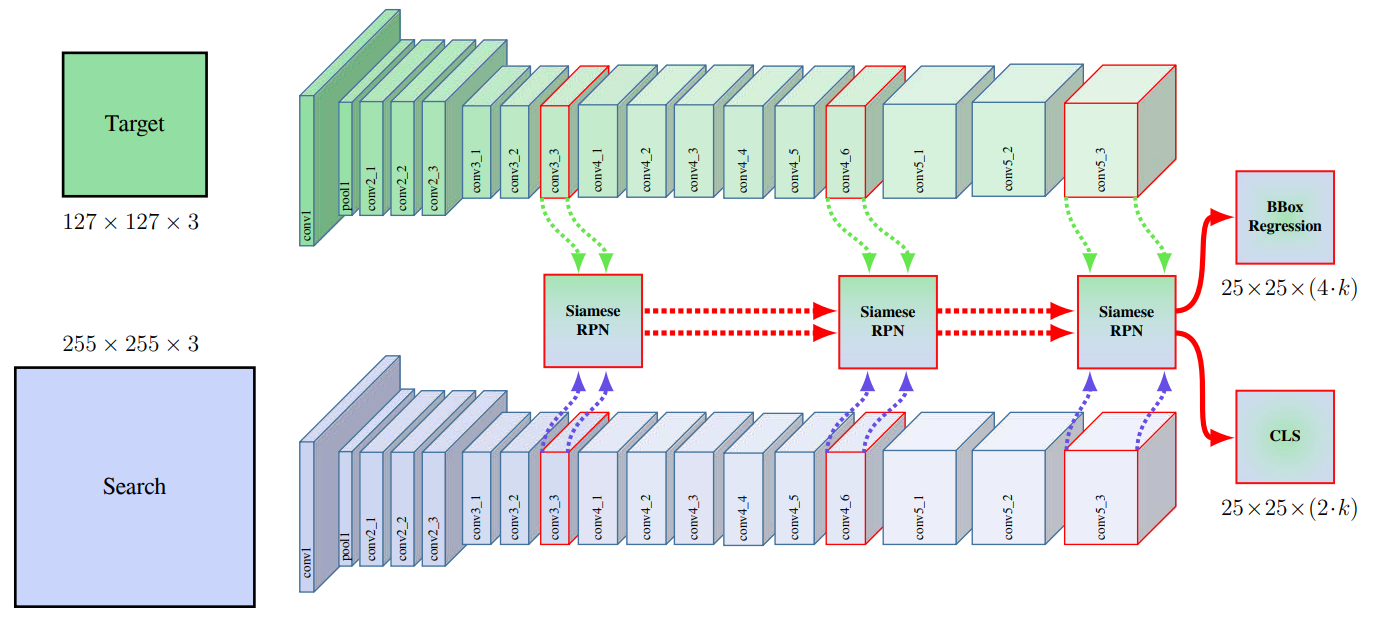
\includegraphics[width=0.75\textwidth]{Img/related/SiamRPN++.png}
\caption{SiamRPN++}
\end{figure}

\begin{figure}
\centering
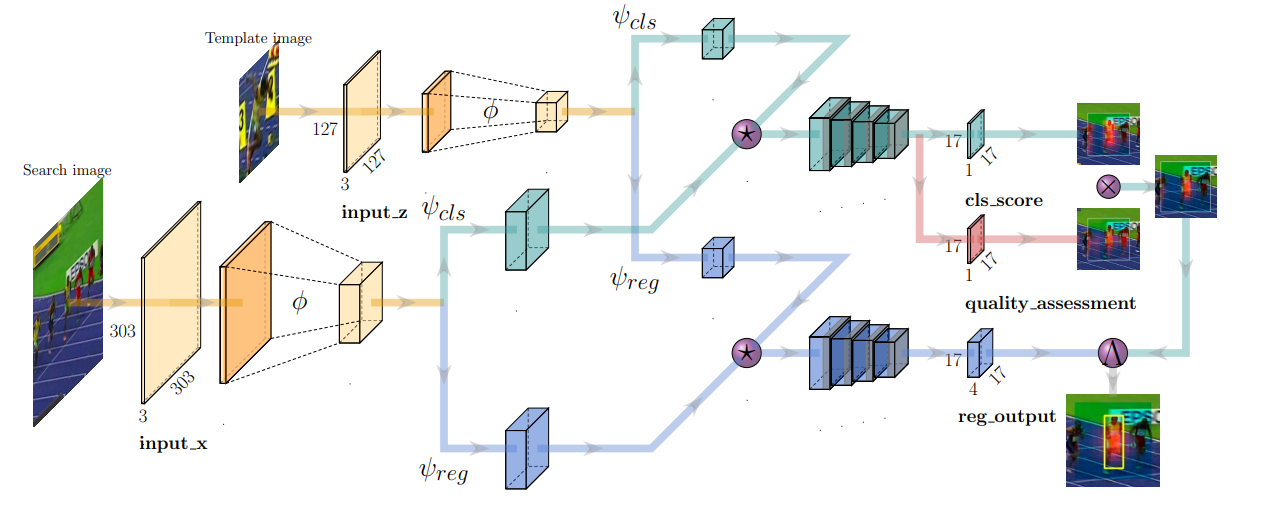
\includegraphics[width=0.75\textwidth]{Img/related/SiamFC++.png}
\caption{SiamFC++}
\end{figure}

\section{本文涉及的视频目标跟踪数据库}
为了衡量不同视频目标跟踪算法的效果,需要形成公平、统一的衡量标准。世界上许多研究机构都发布了不同的视频目标跟踪数据库用于测试各种视频目标跟踪算法的性能。目前针对视频目标跟踪任务常用的数据集有  Object Tracking Benchmark(简称 OTB)\cite{OTB} 数据集、Visual Object Tracking(简称 VOT)\cite{VOT} 挑战赛数据集大规模通用视觉目标跟踪数据集 GOT-10k \cite{GOT-10k} 等。
引入了视觉跟踪基准数据集,以提供对单对象跟踪算法的公正和标准化的评估。这些基准主要根据通用或鸟瞰跟踪应用程序进行分类,同时提供短期或长期情况。这些数据集包含各种序列,框架,属性和类(或类)。这些属性包括照度变化(IV),比例变化(SV),遮挡(OCC),变形(DEF),运动模糊(MB),快运动(FM),面内旋转(IPR),面外旋转(OPR),视线外(OV),背景杂波(BC),低分辨率(LR),宽高比变化(ARC),相机运动(CM),完全遮挡(FOC),部分遮挡(POC) ,相似物体(SIB),视点变化(VC),光(LI),表面覆盖(SC),镜面度(SP),透明度(TR),形状(SH),运动平滑度(MS),运动相干性(MCO) ,混乱(CON),低对比度(LC),变焦相机(ZC),长时间(LD),阴影变化(SHC),闪光灯(FL),弱光(DL),相机抖动(CS),旋转(ROT) ),快速背景变化(FBC),运动变化(MOC),物体颜色变化(OCO),场景复杂度(SCO),绝对运动(AM),尺寸(SZ),相对速度(RS),干扰物(DI),长度(LE),快速摄像机运动(FCM),物体运动(OM),物体模糊(OB),大遮挡(LOC),小物体(SOB),遮挡背景杂波(O-B),旋转遮挡(O-R)和长期跟踪(LT)。表VI比较了应用程序,方案,特征,无监督训练中缺少的标记数据以及单个对象跟踪数据集的重叠。通过不同的评估协议,现有的视觉跟踪基准可以评估现实场景中跟踪器的准确性和鲁棒性。统一的评估协议有助于直观跟踪器的直接比较和开发。下面简要介绍最流行的视觉跟踪基准数据集和评估指标。 A.短期跟踪数据集1)通用对象跟踪:作为最早的对象跟踪基准之一,OTB2013 [218]由完全注释的视频序列开发,以解决基于一些视频序列或初始序列不一致的报告跟踪结果的问题条件或参数。 OTB2015 [219]是扩展的OTB2013数据集,旨在实现无偏性能比较。为了比较视觉跟踪器在颜色序列上的性能,Temple-Color 128(TColor128或TC128)[224]收集了129个完全注释的视频序列,其中有78个与OTB数据集不同。收集了阿姆斯特丹普通视频(ALOV)数据集[42],以涵盖各种视频序列和属性。通过强调具有挑战性的视觉跟踪场景,ALOV数据集包括304个短视频和10个长视频。这些视频片段是从真实的YouTube视频中选择的,难度级别为13。 ALOV的视频已根据其属性之一进行了分类(表VI),尽管在OTB数据集中,每个视频都具有几种视觉属性。 VOT数据集[34]-[40]受到大型数据集不等式的启发,它提供了一个与现有数据集不同且足够小的数据集,并通过可旋转的BB和视觉属性对每帧进行了注释。为了快速而直接地评估不同的视觉跟踪方法,VOT包含视觉跟踪交换(TraX)协议[252],该协议不仅可以准备数据,运行实验并执行分析,还可以检测跟踪失败(即失去目标),并且每次失败后重新初始化跟踪器,以评估跟踪的鲁棒性。尽管野外有一些小型且饱和的跟踪数据集(主要用于对象检测任务),但已提出大规模TrackingNet基准数据集[228]以正确地提供给深层视觉跟踪器。它提供了500个原始视频,超过1400万个垂直BB注释,及时的密集注释数据,丰富的对象类别分布以及YouTube采样视频的真实场景,可用于野外跟踪的视频。为了跟踪行人和刚性物体,已向NUS人和刚性物体(NUS-PRO)数据集[225]提供了来自YouTube的365个视频序列,这些视频序列主要是由移动摄像机捕获的,并注释了每个帧的被遮挡对象的水平,没有遮挡,部分遮挡和完全遮挡标签。通过更高帧频(240 FPS)的摄像机,对速度(NfS)数据集的需求[226]提供了来自真实场景的视频序列,以系统地研究与视觉跟踪器实时分析相关的权衡带宽约束。这些视频可以通过手持式iPhone / iPad摄像机录制,也可以通过YouTube视频录制。两个长期序列数据集,即TinyTLP和TLPattr [232],是从长期TLP数据集中获得的。对于每个序列,已经指定了一个视觉属性来调查各种挑战。大型的高多样性数据集称为GOT-10k [231],包括一万多个视频,分为563类运动对象和87类运动,以尽可能覆盖现实情况中的各种挑战性模式。 GOT-10k具有信息丰富的连续属性,包括缺少标签,这些属性表明目标在框架中不存在。 最后,TracKlinic [233]引入了一个工具包(从OTB2015,TC128和LaSOT收集),该工具包每个序列仅包含一个具有挑战性的因素来评估视觉跟踪器。 它还提供了两个具有挑战性的O-B和O-R属性,包括背景杂波和旋转的遮挡。 2)空中物体跟踪:考虑到广泛的应用范围,近年来已经开发了从空中物体跟踪的方法。(UAV123)[221]提供了一个稀疏的低空鸟瞰跟踪数据集,其中包含由专业级飞行机器人,安装在小型低成本飞行机器人和模拟器上的板载摄像机捕获的逼真的和合成的高清视频序列。无人机跟踪基准(DTB)[227]是由飞行的机器人或无人机捕获的数据集,其中包括RGB视频,由于摄像机突然移动,其目标位置发生了很大的位移。 BUAA-PRO数据集[230]是基于分段的基准数据集,用于解决BB中不可避免的非目标元素的问题。它利用了基于级别的遮挡属性的基于分段掩码的版本。 UAVDT数据集[222]提供了具有高对象密度场景(例如,不同的天气条件,摄像机视图,飞行高度)的鸟瞰图数据集,重点关注行人和车辆。此外,VisDrone数据集[223],[235]包括现实世界中不同无人机平台捕获的视频。对于小物体跟踪,Small90数据集[236]呈现了大部分从其他视觉跟踪数据集中收集的航拍视频。通过添加22个更具挑战性的序列,基于Small-90数据集形成了Small-112数据集[236]。 B.长期跟踪数据集1)通用对象跟踪:为了长期跟踪频繁消失的目标,OxUvA数据集[229]包括来自YouTubeBoundingBoxes(或YTBB)[243]的14小时视频,以提供开发和具有连续属性的测试集。另外,它提供了缺少的标签,表明某些帧中不存在目标。 TLP数据集[232]还从YouTube收集了每个序列持续时间更长的高分辨率视频,这为研究跟踪一致性提供了可能。但是,目标消失在TLP数据集中并不常见。因此,LTB-35 [234]提出了一个丰富的长期数据集,具有一致的目标消失(每个视频平均十二个消失)。大规模的单一对象跟踪(LaSOT)[220]已经被开发来解决现有数据集的问题,例如小规模,缺乏高质量,密集注释,短视频序列和类别偏差。对象类别来自ImageNet和一些视觉跟踪应用程序(如无人机),每个类别具有相同数量的视频。训练和测试子集分别包括1120(2.3M帧)和280(690K帧)视频序列。 2)空中物体跟踪:作为UAV-123数据集的父集,UAV20L是一个空中监视数据集,包括一个连续拍摄的视频序列。它由可容忍的遮挡组成,并为小物体跟踪提供了困难的场景。此外,VisDrone-2019 / 2020L数据集[223]包含25个具有微小目标的具有挑战性的序列(即白天/晚上的12/13个视频)。% Deep Learning for Visual Tracking: A Comprehensive Survey

\subsection{OTB 视频目标跟踪数据集}
OTB 使用50个完全注释的序列构建跟踪数据集,以方便跟踪评估。
OTB 定义了 11 中视觉属性并对视频序列进行了分类标注。这些属性包括:括光照变化、低分辨率、尺度变化、背景干扰、目标遮挡、目标出画面、非刚性形变、平面内旋转、平面外旋转、运动模糊以及快速运动。
在 OTB 中,使用 presicion 和 success rate 进行定量分析。此外,从两个方面评估跟踪算法的鲁棒性。

\textbf{精度图} 在衡量跟踪算法精确度评价指标中,一种广泛使用的方法是中心位置误差,其定义是:预测的目标中心位置与人工标记的真实目标中心位置的平均欧几里得距离。然后,使用一个视频序列的所有帧的平均中心位置误差来代表该视频的总体性能。但是,当跟踪器丢失目标时,预测的位置可能是随机的,因此上述平均误差值可能无法正确衡量跟踪性能。最近,采用精度图来衡量整体跟踪性能。它显示了估计位置在地面真相的给定阈值距离内的帧的百分比。作为每个跟踪器的代表精度得分,我们使用阈值=20像素的得分。
\textbf{成功图} 另一个评估指标是边界框重叠。给定预测的边界框和真实边界框,重叠分数定义为这两个边框的交并比。为了衡量跟踪器在由多帧组成的视频上的性能,我们计算边框重叠大于给定阈值的帧的数量。成功图反映了成功的帧数在给定阈值(0到1之间)的比率。使用特定阈值(例如to = 0.5)的一个成功率值进行跟踪器评估可能不公平或不典型。 相反,我们使用每个成功图的曲线下面积(AUC)对跟踪算法进行排名。

\subsection{VOT 视频跟踪数据集}
VOT 挑战的目标是用户在序列的第一个图像中手动初始化跟踪器的情况。万一跟踪器发生故障(例如,偏离目标),则用户将在故障图像处重新初始化跟踪器。因此,需要跟踪器为序列的每个帧预测目标的单个边界框。通过将预测的边界框与地面真值注释进行比较,可以自动检测到故障,如果重叠为零,则宣布为故障。
为了更好地了解跟踪器的性能,我们为每个选定序列中的每个帧手动或半手动标记了五个视觉属性,这些属性反映了外观退化的特定挑战:(i)遮挡,(ii)照明变化,( iii)运动变化,(iv)尺寸变化,(v)摄像机运动。如果特定帧不对应于五个降级中的任何一个,我们将其表示为(vi)未降级。
基于最近对广泛使用的性能指标的分析[44],我们选择了两个正交指标:(i)准确性和(ii)鲁棒性。精度测量跟踪器预测的边界框与地面真值边界框的重叠程度。另一方面,鲁棒性衡量的是跟踪器在跟踪过程中失去目标的次数。

\subsection{GOT-10k 视频跟踪数据集}
GOT-10k建立在WordNet结构的骨干基础上[1],它填充了563多个运动对象和87个运动模式,旨在为开发与类无关的通用短期跟踪器提供统一的培训和评估平台。
GOT-10k提供了10,000多个视频片段,并带有超过150万个手动标记的边界框,从而可以对深度跟踪器进行统一培训和稳定评估。
GOT-10k首次引入了用于跟踪器评估的单发协议,其中培训和测试课程是零重叠的。该协议避免了对熟悉对象的偏倚评估结果,并促进了跟踪器开发的一般化。
我们构建了一个大型的稳定测试集,其中包括420个视频,这些视频属于84个对象类和31个运动类。我们选择广泛使用的平均重叠(AO)和成功率(SR)作为指标。 AO表示所有地面和估计边界框之间的重叠的平均值,而SR表示重叠超过阈值(例如0.5)的成功跟踪帧的百分比。